\documentclass{cmn}
\usepackage{amsmath}
\usetikzlibrary{circuits.logic.US}

\begin{document}
  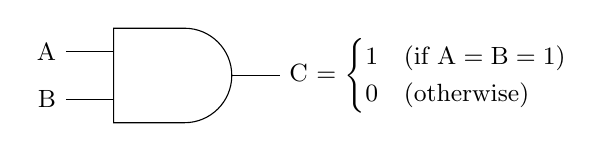
\begin{tikzpicture}
    \node[and gate US,draw,logic gate inputs=nnn,logic gate input sep=3mm] (A) {};
    \coordinate (InA)  at ([xshift=-6mm]A.input 1);
    \coordinate (InB)  at ([xshift=-6mm]A.input 3);
    \coordinate (OutC) at ([xshift=+6mm]A.output);

    \node[left]  at (InA)  {\small A};
    \node[left]  at (InB)  {\small B};
    \node[right] at (OutC) {\small C ={}
      $\begin{cases}
        \text{1}  &\text{(if $\text{A} = \text{B} = 1$)} \\
        \text{0} &\text{(otherwise)}
      \end{cases}$
    };

    \draw (InA) -- (A.input 1);
    \draw (InB) -- (A.input 3);
    \draw (A.output) -- (OutC);
  \end{tikzpicture}
\end{document}
